% ---------------------------------------------------------------------------- %

\PassOptionsToPackage{dvipsnames}{xcolor}

\documentclass[acmsmall,nonacm,screen]{acmart}

\usepackage[utf8]{inputenc}
\usepackage[T1]{fontenc}

\usepackage{minted}
\usepackage{algorithm}
\usepackage{algpseudocode}
\usepackage{varwidth}
\usepackage{array}
\usepackage{multirow}
\usepackage{stackengine}
\usepackage{blindtext}
\usepackage{enumitem}
\usepackage[portuges]{babel}
\usepackage[toc,page]{appendix}

% ---------------------------------------------------------------------------- %
% configuration

% configure template

\makeatletter
\let\@authorsaddresses\@empty
\makeatother

\makeatletter
\let\ftype@table\ftype@figure
\makeatother

\makeatletter
\setlength{\@fptop}{0pt plus 1fil}
\setlength{\@fpbot}{0pt plus 1fil}
\makeatother

\setlength{\intextsep}{10pt}
\setlength{\textfloatsep}{10pt}

\captionsetup[figure]{name={Figure}}

\setlist{nosep}

% ---------------------------------------------------------------------------- %
% utilities

\makeatletter
\newcommand{\gobblepars}{\@ifnextchar\par{\expandafter\gobblepars\@gobble}{}}
\makeatother

\renewcommand{\paragraph}[1]{%
  \vspace*{.5\baselineskip}%
  \noindent\textbf{#1.} %
  \gobblepars%
  }

\newcommand{\mynote}[3]{%
    {\color{black}%
        \fbox{\bfseries\sffamily\scriptsize#1}%
        {\small$\blacktriangleright$\textsf{\emph{\color{#2}{#3}}}$\blacktriangleleft$}%
    }%
  }

% ---------------------------------------------------------------------------- %
% document

\begin{document}

\title{Engenharia Web 19/20 -- Arquitetura do projeto Sidewalk Monitoring System}
\makeatletter \renewcommand{\shortauthors}{\@title} \makeatother

\begin{abstract}
\large
\vspace*{-.8\baselineskip}
José Pereira (A82880), Ricardo Petronilho (A81744)
\vspace*{.4\baselineskip}
\par \noindent \today
\vspace*{.25\baselineskip}
\end{abstract}

\maketitle


\section{Introdução}
\hspace{5mm} Neste relatório apresenta-se a proposta de Arquitetura para o projeto Sidewalk Monitoring System, proposto pela equipa docente da unidade curricular de Engenharia Web.

\hspace{5mm} Inicialmente será apresentada uma modelação dos dados/domínio do problema. De seguida a listagem dos micro serviços necessários para esta arquitetura. Por fim, apresentação/explicação da arquitetura proposta para o Sidewalk Monitoring System.

\section{Modelação do Problema (Domínio)}

\hspace{5mm} Na fase anterior do projeto, implementação estrutural do projeto em \textbf{WebRatio}, o modelo lógico proposto, que reflete o modelo de domínio, foi o seguinte.

\begin{figure}[H]
    \centering
    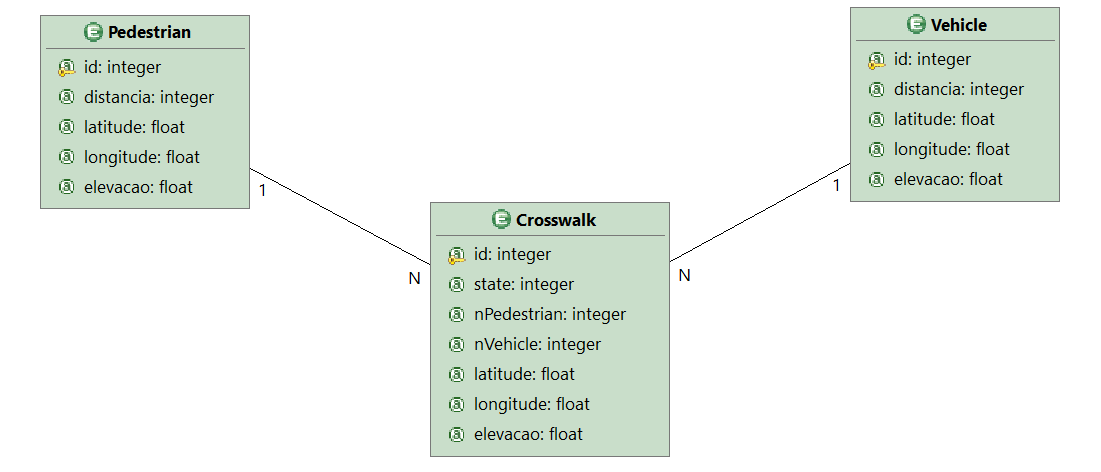
\includegraphics[scale=0.5]{images/modelo-logico-inicial.png}
    \caption{Modelo lógico inicial.}
    \label{img:modelo-logico}
\end{figure}

\hspace{5mm} O modelo lógico faz sentido quando se trata de um sistema simplista que apenas interage com uma única base de dados. No entanto nesta segunda fase, na qual foi desenvolvida a arquitetura, o grupo apercebeu-se que tal não se verifica uma vez que o sistema está dividido em vários \textbf{micro-serviços, sendo que cada um deles necessita de uma base de dados privada (ou de tabelas privadas na mesma base de dados)} tornando assim impossível a utilização do modelo lógico proposto em cima.

\hspace{5mm} Na próxima secção, juntamente com a descrição de cada micro-serviço será referido o modelo lógico \textbf{redefinido} que cada um utiliza.

\section{Micro Serviços}

\begin{figure}[H]
    \centering
    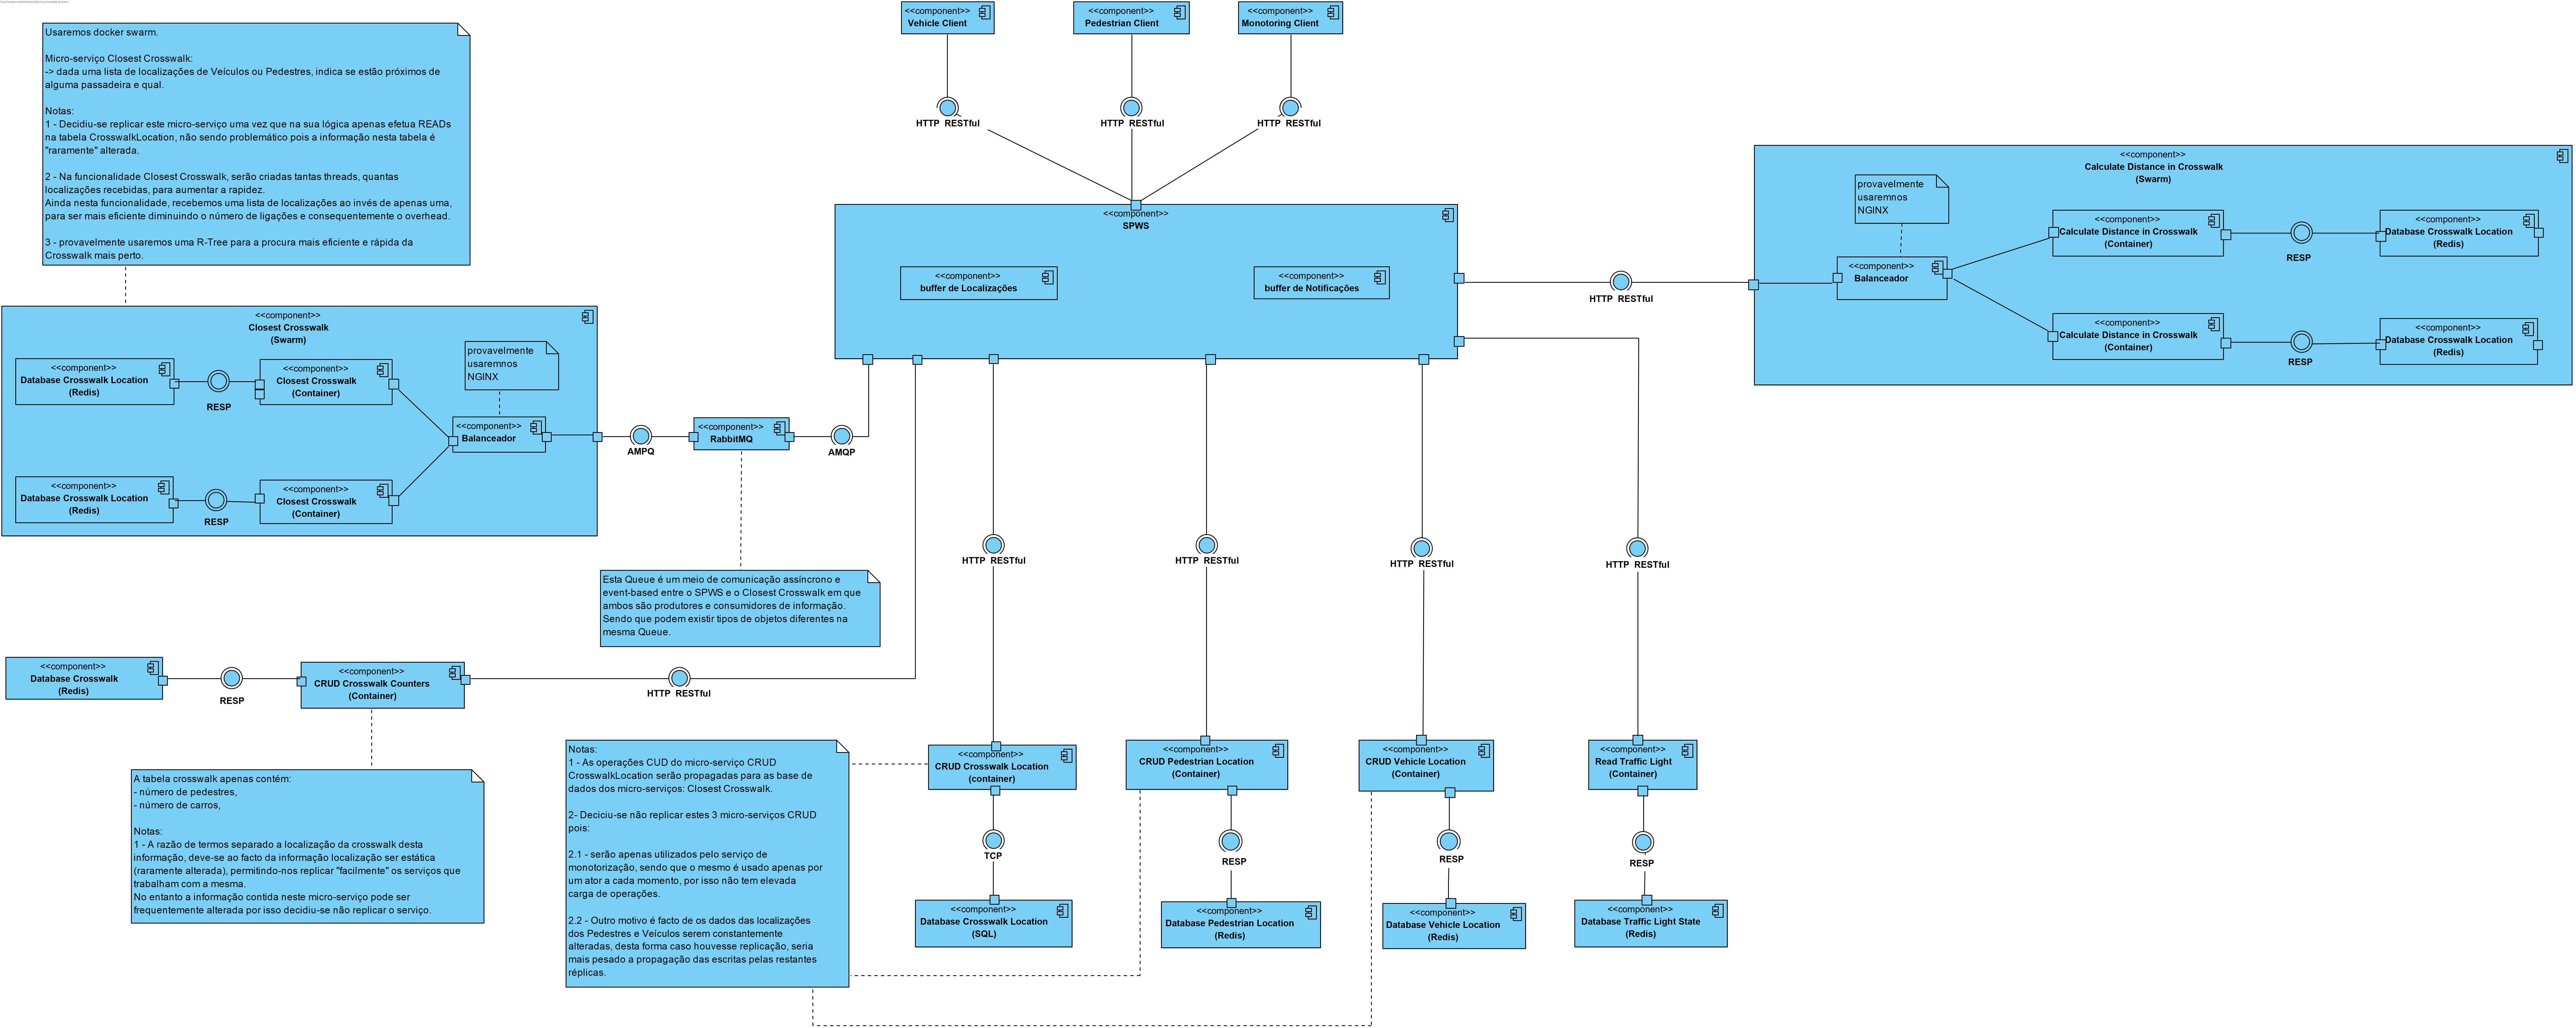
\includegraphics[scale=0.19]{images/Arquitetura.png}
    \caption{Diagrama de componentes.}
\end{figure}

\hspace{5mm} Nesta secção são descritos os micro-serviços integrados na arquitetura, bem como as decisões que levaram à sua criação e estruturação dos mesmos. 

\hspace{5mm} Foram definidos os seguintes micro-serviços:
\newline

\begin{itemize}
    \item Closest Crosswalk (redis, replicado)
    \item CRUD Crosswalk Counters (redis)
    \item CRUD Crosswalk Location (SQL)
    \item CRUD Pedestrian Location (redis)
    \item CRUD Vehicle Location (redis)
    \item Read traffic light (redis)
    \item Calculate distance in Crosswalk (redis, replicado)
\end{itemize}

\subsection{Closest Crosswalk}
\label{closest_crosswalk} 

\hspace{5mm} O micro-serviço Closest Crosswalk é responsável por \textbf{indicar a passadeira mais próxima de uma dada localização}. 

\hspace{5mm} Visto que a lógica de procura da respetiva passadeira pode ser um processo exaustivo e com elevada complexidade o grupo identificou possíveis algoritmos eficientes sendo que o ideal seria o uso de \href{https://en.wikipedia.org/wiki/R-tree}{R-Trees}. No entanto existem outras alternativas mais simples (mas possivelmente menos eficientes) tais como a separação do total de passadeiras em N grupos e utilizar N Threads que exaustivamente efetuam a procura.

\hspace{5mm} Concluiu-se que a \textbf{resposta em tempo útil} deste micro-serviço é fundamental para a notificação atempada tanto dos pedestres como dos veículos desta forma para aumentar a rapidez de processamento e \textbf{assegurar que com o aumento de carga o micro-serviço continua a ter tempos de resposta eficientes ou mesmo que não falha} decidiu-se utilizar um cluster usando a tecnologia \href{https://docs.docker.com/engine/swarm/}{Docker Swarm}. Sendo o mesmo um conjunto de máquinas virtuais ou físicas que implementam um cluster em que uma máquina denominada por \textbf{master}, após pré-configurada, faz a gestão automática dos micro-serviços e respetivas réplicas, fornecidos pelas restantes máquinas denominadas por \textbf{slaves}. O número concreto de réplicas e máquinas a utilizar não está, ainda, definido uma vez que é necessária a realização de \textbf{testes de carga} quando existir uma implementação prática do micro-serviço. Para a realização do \textbf{balanceamento de pedidos entre as réplicas} o grupo decidiu integrar a tecnologia \href{https://www.nginx.com/}{NGINX} no cluster.

\hspace{5mm} Tal como referido na secção anterior, foi necessária a alteração do modelo lógico para a distribuição e replicação dos dados nos micro-serviços. O micro-serviço Closest Crosswalk necessita apenas da localização de todas as passadeiras, desta forma o modelo lógico utilizado apenas contém as coordenadas (latitude, longitude e altitude) das passadeiras. Concluiu-se que a localização de cada passadeira são dados, pela sua natureza, \textbf{alterados momentaneamente}, desta forma serão efetuadas, \textbf{maioritariamente, leituras} sobre os mesmos por isso a replicação destes dados torna-se facilitada. Sendo que \textbf{cada réplica do micro-serviço contém uma réplica dos dados} no seu armazenamento de dados privado. Caso exista alteração dos dados, mesmo que raramente, \textbf{a alteração é propagada para todas as réplicas}. A tecnologia a utilizar para o armazenamento de dados é o \href{https://redis.io/}{Redis} uma vez que é rápida por conter os dados em RAM.

\subsection{CRUD Crosswalk Counters}
\hspace{5mm} O micro-serviço CRUD Crosswalk Counters é responsável pelas funcionalidades \textbf{CRUD}(Create, Read, Update e Delete) da tabela Crosswalk referente aos contadores de \textit{pedetrians/vehicles}.

\hspace{5mm}Tal como já foi referido anteriormente, o modelo lógico proposto inicialmente foi afetado por forma a distribuir a lógica por micro serviços. Dessa forma, a tabela com a informação da Crosswalk presente neste micro-serviço, ao contrário do que se pode observar na figura \ref{img:modelo-logico}, apenas contém os atributos \textbf{id} da crosswalk, e os contadores de \textit{pedestrians} e \textit{vehicles} diários, não contendo a localização, e estado da traffic light da mesma. A razão pela qual foi feita esta divisão de atributos deve-se ao facto da localização da crosswalk ser "raramente" alterada, no entanto, frequentemente  \textbf{acedida}, ou seja, caso o read dessa informação ficasse neste micro-serviço iria "pesá-lo" ainda com mais pedidos. Do mesmo modo, a informação do estado da \textit{traffic light} foi separada desta informação (a informação da localização e estado da traffic light da crosswalk, bem como os micro-serviços responsáveis por essas informações serão abordados mais aditante).

\hspace{5mm} O armazenamento de dados neste micro-serviço efetua-se utilizando um \href{https://redis.io/}{Redis}, devido à necessidade de rapidez nos tempos de resposta. No entanto, o \href{https://redis.io/}{Redis} consiste num sistema \textit{non-blocking}, isto é, escritas não bloqueiam leituras, não sendo crítico (ao contrário por exemplo das notificações dos clientes) para o sistema, pois caso o número de \textit{pedestrians}/\textit{vehicles} apresentado na monitorização não seja o mais atualizado, o mesmo será no próximo refresh da mesma.

\subsection{CRUD Crosswalk Location}
\label{traffic_light} 

\hspace{5mm} O micro-serviço CRUD Crosswalk Location é responsável pelas funcionalidades \textbf{CRUD}(Create, Read, Update e Delete) da tabela Crosswalk referente à localização da crosswalk.

\hspace{5mm} Tal como já foi dito anteriormente, esta informação foi separada tanto da informação dos contadores, bem como da traffic light. A razão pela qual foi separada, deve-se à "raridade" (se pensarmos que se cria uma crosswalk a cada semana, isso será pouco para o sistema) de escritas efetuadas da localização das crosswalks, bem como do elevado número de leituras efetuadas da mesma. Assim evita-se um único micro serviço CRUD de toda a informação da crosswalk, o qual ficaria muito "pesado".

\hspace{5mm} Outra responsabilidade deste serviço será de em cada alteração/adição de uma nova crosswalk (localização), propagar esses dados para todos os serviços onde exista a informação de localização das mesmas, tais como, \textbf{Closest Crosswalk} e \textbf{Calculate Distance in Crosswalk}.

\hspace{5mm} A base de dados utilizada será \textbf{SQL}, visto que, se pretende persistir as localizações das crosswalks.

\subsection{CRUD Pedestrian Location \& CRUD Vehicle Location}

\hspace{5mm} A razão pela qual abordar-se-á estes dois micro serviços em conjunto, deve-se ao facto de serem bastante semelhantes, no entanto, para informações/dados diferentes, sendo respetivamente para a informação do \textbf{Pedestrian} e \textbf{Vehicle}.

\hspace{5mm} Os micro-serviços \textbf{CRUD Pedestrian Location} \& \textbf{CRUD Vehicle Location} são responsáveis pelas funcionalidades \textbf{CRUD} (Create, Read, Update e Delete) da informação (localização e id) respetivamente do \textbf{Pedestrian} e \textbf{Vehicle}.

\hspace{5mm} Nestes micro serviços utilizou-se \href{https://redis.io/}{Redis}, que apesar de ser \textit{non-blocking}, ou seja, as escritas não bloqueiam as leituras, significa que dados podem ser lidos durante escritas tal como já foi referido anteriormente. Dado que, a localização dos \textbf{Pedestrians} e \textbf{Vehicles} consiste num dado crítico, ou seja, a consistência/integridade do seu valor torna-se importante, desta forma, pode-se pensar ser arriscado utilizar \href{https://redis.io/}{Redis}, pois quando houvesse uma leitura de uma localização a mesma pode não ser a mais atualizada. 

\hspace{5mm} No entanto, apesar da localização ser um dado crítico, quando existe necessidade de notificar o \textbf{pedestrian} ou \textbf{vehicle}, efetua-se o mesmo no momento em que se identifica o "perigo". Isto é, após o micro serviço \textbf{Closest Crosswalk} referido anteriormente , identificar que uma das entidades encontra-se em "perigo", notifica-o nesse mesmo momento, e só de seguida escreve a informação, para que outros serviços ou funcionalidades a possam usar. Desta forma, a utilização de \href{https://redis.io/}{Redis} neste dado crítico não influencia nessas situações.


\subsection{Read Traffic Light}

\hspace{5mm} O micro-serviço Read Traffic Light é responsável por \textbf{indicar o estado do traffic light de uma determinada passadeira}. 

\hspace{5mm} Tal como referido na secção \ref{traffic_light}, inicialmente a informação do taffic light estava anexada num único serviço que continha, também, os contadores de pedestres e veículos. No entanto esse serviço seria \textbf{sobrecarregado uma vez que era utilizado constantemente} tanto para leituras na monotorização bem como para escritas quando se detetava a existência de pedestres ou veículos numa passadeira e ainda eram efetuadas leituras para implementar o requisito de notificar o estado do traffic light tanto aos pedestres como veículos. 

\hspace{5mm} Na implementação deste último requisito os atores devem ser notificados em tempo útil assim a separação em dois micro-serviços, sendo um responsável pelo CRUD dos contadores e outro apenas para leitura do traffic light torna-se necessária para que exista \textbf{balanceamento de carga, ficando a leitura do estado do traffic light mais disponível e por isso com tempo de resposta menor}.

\hspace{5mm} Visto que o estado do traffic light, pela sua natureza, é constantemente alterado, torna-se complexa a replicação destes dados, no entanto para que a leitura seja mais rápida decidiu-se utilizar a tecnologia \href{https://redis.io/}{Redis}.


\subsection{Calculate distance in Crosswalk}

\hspace{5mm} O micro-serviço Calculate distance in Crosswalk é responsável por indicar a distância de um pedestre ou veículo a uma passadeira dado a localização dos atores e o identificador da respetiva passadeira.

\hspace{5mm} Visto que este micro-serviço é apenas utilizado na monotorização, decidiu-se enviar apenas o identificador da passadeira e não a localização da mesma pois podem ser efetuados \textbf{muitos pedidos de cálculos de distância para a mesma passadeira (enquanto está a ser observada) sendo o identificador menos dados a ocupar na rede}.

\hspace{5mm} Desta forma este micro-serviço necessita de armazenar a localização de todas as passadeiras, sendo o mesmo feito utilizado a tecnologia \href{https://redis.io/}{Redis}. 

\hspace{5mm} Tal como na secção \ref{closest_crosswalk} concluiu-se que a localização de cada passadeira são dados, pela sua natureza, \textbf{alterados momentaneamente}, desta forma serão efetuadas, \textbf{maioritariamente, leituras} sobre os mesmos por isso a replicação destes dados torna-se facilitada. Sendo que \textbf{cada réplica do micro-serviço contém uma réplica dos dados} no seu armazenamento de dados privado. Caso exista alteração dos dados, mesmo que raramente, \textbf{a alteração é propagada para todas as réplicas}.

\hspace{5mm} Analogamente a replicação do micro-serviço será realziada utilzando \href{https://docs.docker.com/engine/swarm/}{Docker Swarm}.


\section{Serviço SPWS}
\hspace{5mm} A arquitetura implementada consiste numa \textit{Orchestration}, onde o \textbf{SPWS} é o \textbf{Maestro}, gerindo os micro serviços referidos anteriormente.

\hspace{5mm} O SPWS recebe os dados dos clientes (\textbf{Pedestrians} e \textbf{Vehicles}), isto é, as suas localizações, e começa por enviar as mesmas para o micro serviço \textbf{Closest Crosswalk}, no entanto, para uma \textit{queue} que existe entre ambos, de forma a tornar esta funcionalidade \textbf{asíncrona e event-based}, isto é, o \textbf{SPWS} não fica à espera da resposta do mesmo. 

\hspace{5mm} Após o \textbf{Closest Crosswalk} determinar se as localizações recebidas estão no raio de crosswalks, envia a mesma para a queue.

\hspace{5mm} O \textbf{SPWS} recebe as mensagens da queue, enviando imediatamente a notificação para os \textbf{Pedestrians} e \textbf{Vehicles}, sendo que neste último, ainda envia separadamente a notificação do estado da traffic light. O objetivo de enviar as notificações separadas consiste em não "prender"/fazer esperar os \textbf{vehicles} dessa mesma notificação, pois para os mesmo, é mais crucial verificar a presença de pedestres do que o estado da traffic light.

\hspace{5mm} Usufruindo do facto do envio das localizações por parte dos atores são num intervalo de tempo curto, aproveita-se o \textit{Http request}, para, caso haja, uma notificação, ser imediatamente enviada no response, sendo desta forma a comunicação assíncrona visto que não fica à espera.  

\hspace{5mm} Ao mesmo tempo que é efetuada a notificação das entidades é atualizada a localização das mesmas através dos micro-serviços CRUD Pedestrian/Vehicle Location pois esses dados são necessários na monotorização. 
\newline 

\hspace{5mm} Concluindo, o SPWS fornece as seguintes funcionalidades:
\newline

\begin{itemize}
    \item update location: envio da localização por parte dos clientes.
    \item verificação de perigo: dada localização das entidades, verificar se as mesmas estão no raio de uma crosswalk.
    \item notifiação: as entidades em caso de perigo são avisadas do mesmo (\textbf{Pedestrian} e \textit{vehicle}.
    \item monitorização de uma crosswalk: consulta da localização/distância dos \textbf{Pedestrians} e \textbf{Vehicles} na vinhança.
    \item CRUD da informação das crosswalks (localização).
\end{itemize}

\end{document}

% ---------------------------------------------------------------------------- %
